\begin{comment}
Template vir elke funksie
    \paragraph{Funksie naam}
			\begin{description}
			    \item{\textbf{Priority}:} %watter prioriteit dit het: Critical, Important of Nic-to-have
			    \item{\textbf{Service Contract}:}% Wat dit doen
			    \item{\textbf{Pre-conditions}:}%wat moet waar wees voor die funksie sy ding kan doen
    			    \begin{itemize}
    			        \item precondition 1
    			        \item precondition 2
    			    \end{itemize}
			    \item{\textbf{Post-conditions}:} % wat moet waar wees na die funksie sy ding gedoen het
    			    \begin{itemize}
    	    	    \item %post condition 1
    			    \item %post condition2
    			    \end{itemize}
			\end{description}
\end{comment}









\subsection{Application}
		\subsubsection{Scope}
		    The Application is used when entering a meeting. 
		    \begin{itemize}
		    \item The user will hold the mobile device over a node.
		    \item The application will send the device identification and the persons email address to the gateway via the node. 
    		    \begin{description}
    		        \item{\textbf{If permission is granted}:} The background of the application will turn green and the application will take a snapshot of the mobile device's current state and enable the protection. The snapshot is taken so that the mobile Device and application can be restored to its previous state after the meeting.
    		        \item{\textbf{If permission is denied}:} The background of the application will  turn red and the application will do nothing.
    		        
    		    \end{description}
		    \item During the meeting the application check constantly if the protection mode is violated. If so, the protection mode is restored and the mobile device vibrates to alert the user of a possible attack.
		    \item When exiting the meeting the user holds the mobile device over the node again and the mobile device is restored to its previous state.
		    \item{ Overall system layout: 
		    
		    

		
		\begin{figure}[H]
 			 \centering
			  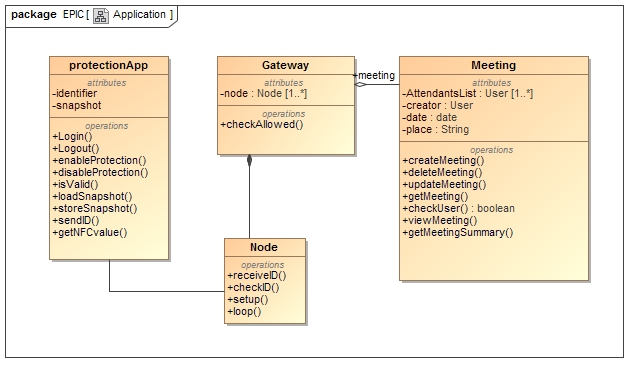
\includegraphics[width=12cm]{ApplicationClass}
		 	 \caption{A Class Diagram of the protection Application, Meeting, Node and Gateway}
		\end{figure}}
		\end{itemize}
       
       
        \subsubsection{Functionality}

		\begin{figure}[H]
 			 \centering
			  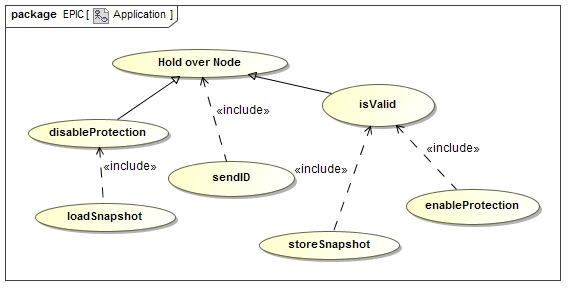
\includegraphics[width=12cm]{ApplicationUseCase}
		 	 \caption{A Use Case Diagram protection Application}
		\end{figure}


    \paragraph{onNewIntent}
			\begin{description}
			    \item{\textbf{Priority}:} Critical%watter prioriteit dit het: Critical, Important of Nic-to-have
			    \item{\textbf{Service Contract}:}This function is called when an Android system intent is triggered. It checks whether the intent was caused by NFC and then parses the NFC message that will check whether the user is allowed to enter the room. If the user is allowed, the store- and loadSnapshot functions are called respectively on whether the user is entering or leaving.% Wat dit doen
			    \item{\textbf{Pre-conditions}:}%wat moet waar wees voor die funksie sy ding kan doen
    			    \begin{itemize}
    			        \item An NFC intent must be triggered by holding the mobile device against a node.
    			        \item Application either in safe or unsafe mode.
      			    \end{itemize}
			    \item{\textbf{Post-conditions}:} % wat moet waar wees na die funksie sy ding gedoen het
    			    \begin{itemize}
    		        \item According to the state of the application, either the LoadSnapshot or StoreSnapshot function should be called.
    			    
    			    \end{itemize}
			\end{description}
	

	    \paragraph{StoreSnapshot}
			\begin{description}
			    \item{\textbf{Priority}:} Critical
			    \item{\textbf{Service Contract}:} This function stores the state of all communication mechanisms and then turns them off to enter \textit{protection mode}.
			    \item{\textbf{Pre-conditions}:}
    			    \begin{itemize}
    			        \item The mobile device must have enough space to store the file with all the states. 
    			        \item The mobile application must be in the unsafe state.
    			    \end{itemize}
			    \item{\textbf{Post-conditions}:} 
    			    \begin{itemize}
    			    \item A file is stored containing the current states of the mobile device's communication mechanisms.
    			    \item All communication mechanisms are turned off.
    			    \item The mobile application's state is switched to safe mode. 
    			    \end{itemize}
			\end{description}
			
	    \paragraph{LoadSnapShot}
			\begin{description}
			    \item{\textbf{Priority}:} Critical%watter prioriteit dit het: Critical, Important of Nic-to-have
			    \item{\textbf{Service Contract}:} This function is an overwritten function. It is used to create the user authentication data and return it when the mobile device is being read from via NFC.% Wat dit doen
			    \item{\textbf{Pre-conditions}:}%wat moet waar wees voor die funksie sy ding kan doen
    			    \begin{itemize}
    			        \item The mobile application should be in the safe state.
    			        \item The connections should not have been toggled on while in safe state.
  
    			    \end{itemize}
			    \item{\textbf{Post-conditions}:} % wat moet waar wees na die funksie sy ding gedoen het
    			    \begin{itemize}
    			    \item The mobile application is switched to unsafe state.
    			    \item The connections of the mobile device are restored based on previous unsafe state.

    			    \end{itemize}
			\end{description}	
			
				
		\paragraph{StoreEmpID}
			\begin{description}
			    \item{\textbf{Priority}:} Critical %watter prioriteit dit het: Critical, Important of Nic-to-have
			    \item{\textbf{Service Contract}:}This function stores a combination of fields entered by the user into a file that is used to with other functions to either retrieve the data if the application is closed and reopen, or send it via NFC to get use as authentication.% Wat dit doen
			    \item{\textbf{Pre-conditions}:}%wat moet waar wees voor die funksie sy ding kan doen
    			    \begin{itemize}
    			        \item The Employee ID text field should not be empty.
    			        \item The ID needs to be valid.
    			        \item The mobile device needs to have enough space to store a file.

    			    \end{itemize}
			    \item{\textbf{Post-conditions}:} % wat moet waar wees na die funksie sy ding gedoen het
    			    \begin{itemize}
    			    \item A file containing the Employee ID is stored to the local mobile device.
    			    \end{itemize}
			\end{description}	
				
		\paragraph{getDeviceId}
			\begin{description}
			    \item{\textbf{Priority}:} Important%watter prioriteit dit het: Critical, Important of Nic-to-have
			    \item{\textbf{Service Contract}:} Used to added an extra security layer to authentication by getting the unique device id.% Wat dit doen
			    \item{\textbf{Pre-conditions}:}%wat moet waar wees voor die funksie sy ding kan doen
    			    \begin{itemize}
    			        \item The mobile device must be a valid device and have a unique id.
    			    \end{itemize}
			    \item{\textbf{Post-conditions}:} % wat moet waar wees na die funksie sy ding gedoen het
    			    \begin{itemize}
    			    \item The state of the mobile application should be unchanged.
    			    \end{itemize}
			\end{description}	
			
		\paragraph{unitTests}
			\begin{description}
			    \item{\textbf{Priority}:} Critical %watter prioriteit dit het: Critical, Important of Nic-to-have
			    \item{\textbf{Service Contract}:}This function uses dummy scenario's to test whether all of the functions work as they should.% Wat dit doen
			    \item{\textbf{Pre-conditions}:}%wat moet waar wees voor die funksie sy ding kan doen
    			    \begin{itemize}
    			        \item The mobile application must be in debugging mode.
    			        \item The mobile application must be in the unsafe state.
    			        \item The mobile application must have enough space to store the results.
    			    \end{itemize}
			    \item{\textbf{Post-conditions}:} % wat moet waar wees na die funksie sy ding gedoen het
    			    \begin{itemize}
    			    \item The mobile application should be in the unsafe state.
    			    \item A file with the unit test results is stored to the mobile device.
    			    \end{itemize}
			\end{description}

				
		\paragraph{setActivityBackgroundColor}
			\begin{description}
			    \item{\textbf{Priority}:} Nice to have%watter prioriteit dit het: Critical, Important of Nic-to-have
			    \item{\textbf{Service Contract}:} This function changes the background colour of the application to visually notify the user if he has been granted access to the meeting room.% Wat dit doen
			    \item{\textbf{Pre-conditions}:}%wat moet waar wees voor die funksie sy ding kan doen
    			    \begin{itemize}
    			        \item The state of the application needs to be changed.
    			    \end{itemize}
			    \item{\textbf{Post-conditions}:} % wat moet waar wees na die funksie sy ding gedoen het
    			    \begin{itemize}
    			    \item The mobile application's background colour should be the new colour.
    			    \end{itemize}
			\end{description}
			
		\paragraph{convertStreamToString}
			\begin{description}
			    \item{\textbf{Priority}:} Nice to have%watter prioriteit dit het: Critical, Important of Nic-to-have
			    \item{\textbf{Service Contract}:} This function helps to convert an input stream of bytes into a \textit{String type} that is used for file reading.% Wat dit doen
			    \item{\textbf{Pre-conditions}:}%wat moet waar wees voor die funksie sy ding kan doen
    			    \begin{itemize}
    			        \item The input stream must be given
    		%	        \item %precondition 2
    			    \end{itemize}
			    \item{\textbf{Post-conditions}:} % wat moet waar wees na die funksie sy ding gedoen het
    			    \begin{itemize}
    			    \item The function returns a String object containing the value of the stream converted to a String data type. 
    		%	    \item %post condition2
    			    \end{itemize}
			\end{description}



